\subsubsection{Proton}

Figure\ref{fig:Proton_Event_Display} shows typical event of proton.
Proton has simple structure of events because proton doesn't decay any particles.
Therefore, it is easy to define stopped point.
We define the hit which has the maximum channel number as stopped point.
However, it should noted that stopped point include fake hit in a proportion because of the influence of cross talk as described in section 6.6.\\

\begin{figure}[htbp]
  \centering
  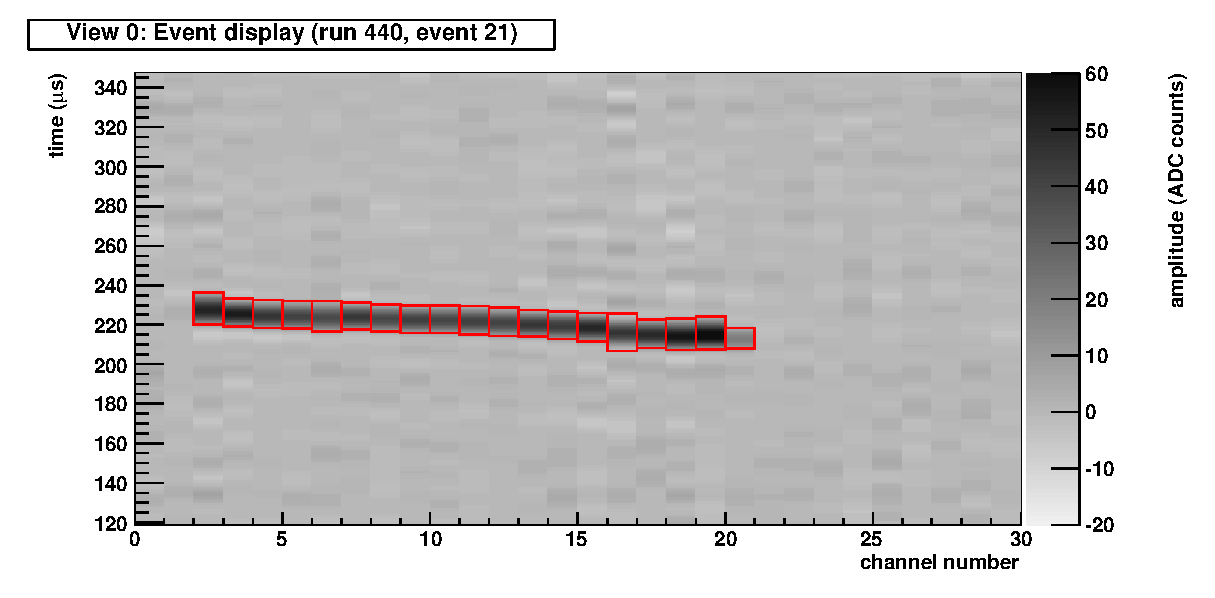
\includegraphics[width=10cm,clip]{fig/Display_run440_ev21.eps}
  \caption{Typical Event Display of Proton}
  \label{fig:Proton_Event_Display}
\end{figure}
